\documentclass[10pt,graphics,aspectratio=169,table]{beamer}
\usepackage{listings}
\usepackage{amsmath}
\usepackage{hyperref}
\usepackage{framed, color}
\usepackage{natbib}
\usepackage{csquotes}

\usetheme{metropolis}
\setbeamertemplate{bibliography item}[text]
\renewcommand{\bibsection}{}

\newcommand{\code}[0]{\lstinline[basicstyle=\ttfamily\color{white}]}
\newcommand{\cbox}[1]{\colorbox{black}{#1}}

\title{WSL - Windows Subsystem for Linux}
\author{Viktor Reusch}
\date{ESE 2019}
\institute{NERD101 - ESE - ifsr - TU Dresden}

\titlegraphic{\hfill
\includegraphics[height=1.25cm]{../logo}}
\begin{document}
\maketitle

\begin{frame}{Outline}
    \tableofcontents
\end{frame}

\section{Why do I need Linux?}
\begin{frame}{Terminal Workflow}
\begin{itemize}
    \item pipes \cbox{\code|\$ tar -tf src.tar \| less|} and redirects \cbox{\code|\$ curl ifsr.de 2> /dev/null|}
    \item editors like \textit{vim} and \textit{emacs}
    \item specialized single purpose programes like \textit{sha256sum}, \textit{cat}, \textit{tail} etc.
    \item package management through \textit{apt}, \textit{pacman}, \textit{yum} etc.
    \item program manuals and help are available with \textit{man}, \textit{tldr} or the \cbox{\code|\--help|} option
    \item standardized directory structure: Filesystem Hierarchy Standard
\end{itemize}
\centering
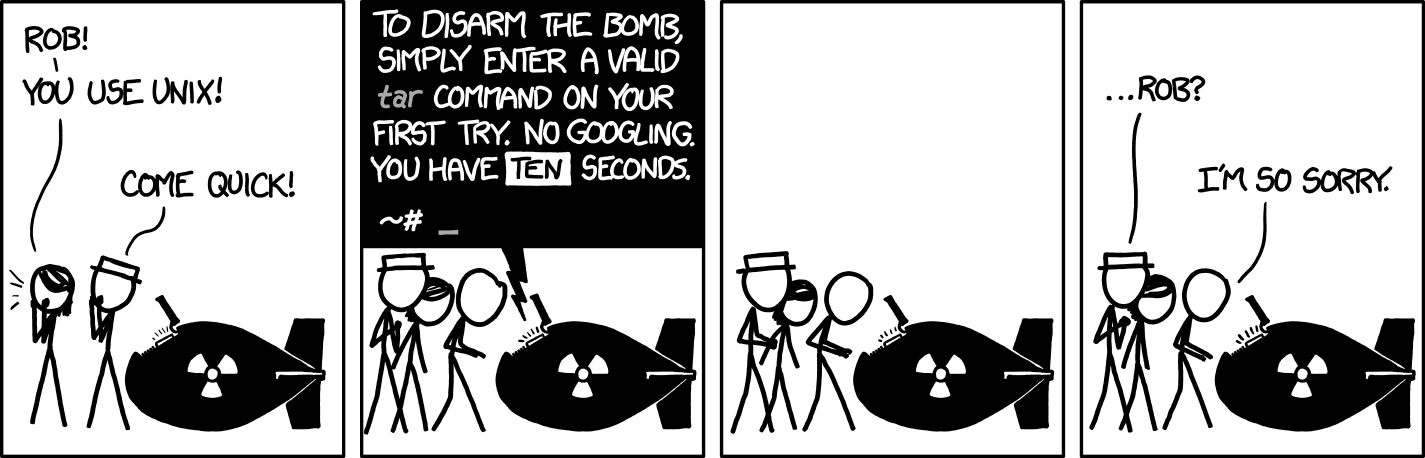
\includegraphics[width=\textwidth]{img/tar.png} \cite{tar}
\end{frame}

\begin{frame}{Studies}
\begin{itemize}
    \item \textit{C} compiler needed for \textit{AUD} in the first semester
    \item \textit{Haskell} and \textit{Prolog} interpreters needed for \textit{Programmierung} in the second semester
\end{itemize}
\end{frame}

\begin{frame}{Developement \& Deployment}
\begin{columns}
    \column{0.7\textwidth}
        \begin{itemize}
            \item building and testing of Linux targeted software
            \item version control systems like \textit{git}
            \item working on a remote server with \textit{ssh}, \textit{sshfs} and \textit{scp}
            \item running services like \textit{nginx}, \textit{sshd} or \textit{systemd}
            \item virtualisation (VM, \textit{Docker}) for development, testing and deployment semester
        \end{itemize}
    \column{0.3\textwidth}
        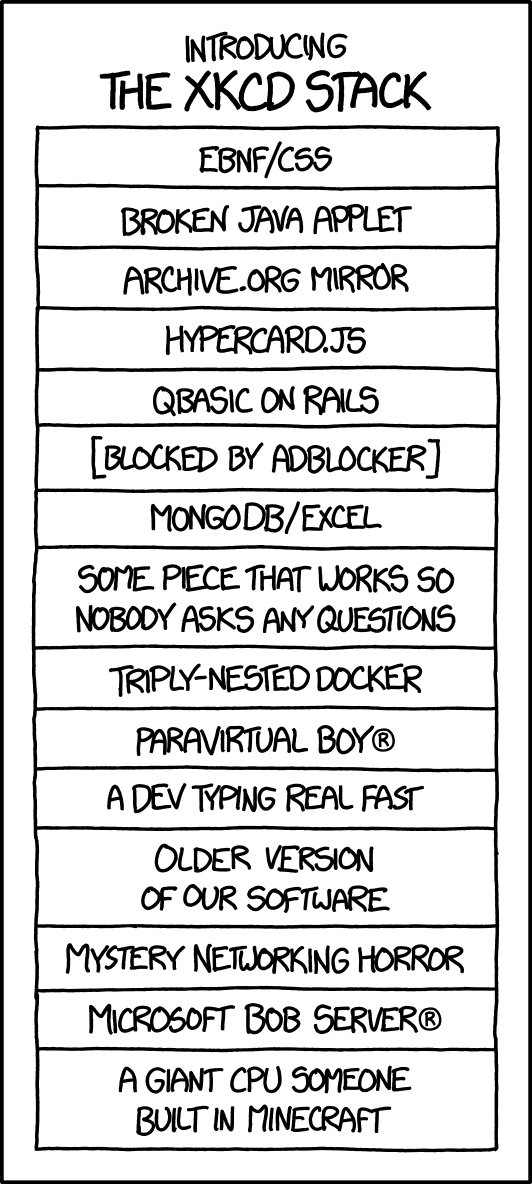
\includegraphics[height=0.75\paperheight]{img/stack} \cite{stack}
\end{columns}
\end{frame}

\section{How do I get Linux?}
\begin{frame}{Dual Boot}
\begin{columns}
    \column{0.7\textwidth}
        \begin{itemize}
            \item two operation systems installed side by side
            \item only one can run at a time
            \item space and partitions needed for both systems
            \item no performance lost
        \end{itemize}
    \column{0.3\textwidth}
        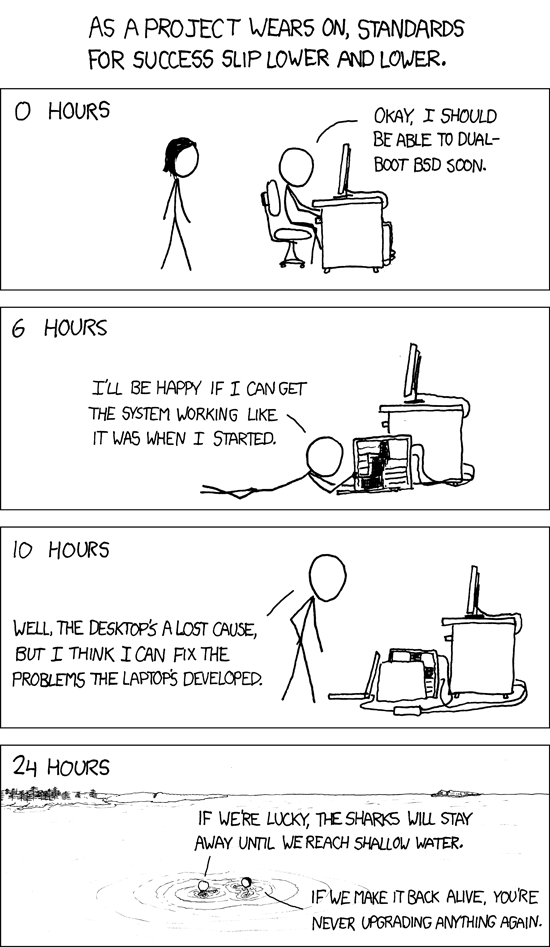
\includegraphics[height=0.75\paperheight]{img/success.png} \cite{success}
\end{columns}
\end{frame}

\begin{frame}{Ports}
\begin{itemize}
    \item typical Linux/BSD software mopdified to run on Windows
    \item \textit{MinGW} (\textit{Minimalist GNU for Windows}) ships ports of \textit{GNU} tools like the \textit{gcc}
    \item \textit{MSYS} supplements this with UNIX tools e.g. \textit{bash} and \textit{grep}
    \item also used by \textit{Git for Windows}
\end{itemize}
\end{frame}

\begin{frame}{VM - Virtual Machine}
\begin{itemize}
    \item visualizes an entire computer to run an complete operation system
    \item allows controlling of a guest OS by a host OS
    \item execution of two operation systems on a single machine
    \item slower than directly running Linux
\end{itemize}
\centering
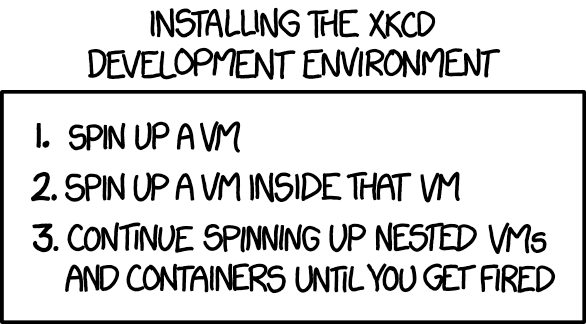
\includegraphics[width=0.5\textwidth]{img/xkcde.png} \cite{xkcde}
\end{frame}

\subsection{What is WSL?}
\section*{What is WSL?}
\begin{frame}{Linux-compatible Kernel Interface}
\begin{itemize}
    \item started Linux binaries are treated differently than Windows binaries
    \item compatibility layer between Linux programs and NT kernel
    \item Linux syscalls are translated by the layer to NT kernel calls
    \item LXSS Manager Service manages linux processes
    \item unmodified Linux user mode binaries can be executed
\end{itemize}
\hfill\cite{overview}
\end{frame}

\begin{frame}{Interoperability}
\begin{itemize}
    \item Linux subsystem with own file system
    \item Windows drives mounted at \cbox{\code|/mnt/[DRIVE\_LETTER]/|}
    \item execution of shell commands from CMD \cbox{\code|> wsl ls -lhA |}
    \item execution of Windows binaries from bash \cbox{\code|\$ nslookup.exe ifsr.de|}
    \item piping to and from WSL \cbox{\code|> tree \| wsl more|}
    \item WSL and Windows share a network connection
    \item WSL can open ports
\end{itemize}
\hfill\cite{interop}
\end{frame}

\begin{frame}{Limitations}
\begin{itemize}
    \item no Linux kernel $\implies$ \textit{mount}, \textit{GUI} and \textit{fuse} unavailable
    \item vitalization like Docker not possible
    \item disc space required for user mode Linux
    \item no direct access of the Linux file system through Windows
    \item only available for Windows 10 64-bit
\end{itemize}
\hfill\cite{wsl2}
\end{frame}

\section{What will come next?}
\begin{frame}{WSL 2}
\begin{columns}
    \column{0.5\textwidth}
        \begin{itemize}
            \item Linux and Windows runs as VM in a type I hypervisor
            \item same technology as Windows Defender sandbox
            \item tightly integrated into Windows like WSL
            \item files transferred over a 9P file server
            \item currently only available in the Insider builds
        \end{itemize}
        \hfill \cite{wsl2}
    \column{0.5\textwidth}
        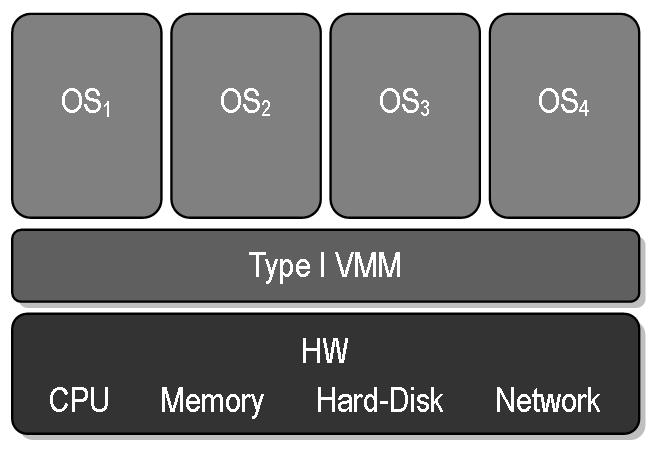
\includegraphics[width=0.9\textwidth]{img/type1.jpg} \cite{type1}
\end{columns}
\end{frame}

\begin{frame}{Improvements}
\begin{itemize}
    \item a real, open source Linux kernel
    \item allows Docker, fuse etc.
    \item runs on a faster \textit{ext4} file system
    \item faster startup than a standard VM
    \item good integration into Windows like execution from CMD and file transfer
\end{itemize}
\hfill\cite{wsl2}
\end{frame}

\section{How do I get WSL?}

\begin{frame}{PowerShell}
\begin{itemize}
    \item open the Windows search
    \item search for \enquote{Windows PowerShell}
    \item left click and \enquote{Run as administrator}
\end{itemize}
\end{frame}

\begin{frame}{Enabling the Feature}
\begin{itemize}
    \item type the following in one line \\
    \cbox{\code|Enable-WindowsOptionalFeature -Online|} \\
    \cbox{\code|-FeatureName Microsoft-Windows-Subsystem-Linux|} \\
    \item press enter
    \item restart the laptop when promted
\end{itemize}
\hfill\cite{installation}
\end{frame}

\begin{frame}{Installing a Distribution}
\begin{itemize}
    \item open the \textit{Microsoft Store}
    \item search for \enquote{Linux}
    \item install a distribution of your choice
    \item start WSL from the CMD \cbox{\code|> wsl|}
    \item follow the initialization steps
\end{itemize}
\hfill\cite{installation}
\end{frame}

\begin{frame}[allowframebreaks]
        \frametitle{References}
        \bibliographystyle{ieeetr}
        \nocite{*}
        \bibliography{ref}
\end{frame}
\end{document}
